\documentclass[12pt,letterpaper]{article}
\usepackage[utf8]{inputenc}
\usepackage{graphicx,textcomp}
\usepackage{natbib}
\usepackage{setspace}
\usepackage{fullpage}
\usepackage{xcolor}
\usepackage[reqno]{amsmath}
\usepackage{amsthm}
\usepackage{fancyvrb}
\usepackage{amssymb,enumerate}
\usepackage[all]{xy}
\usepackage{float}
\usepackage{hyperref}
\usepackage[compact]{titlesec}
\usepackage{dcolumn}
\usepackage{tikz}
\usepackage{multirow}
\usepackage{url}
\usepackage{listings}
\usepackage{pifont}

\definecolor{codegreen}{rgb}{0,0.6,0}
\definecolor{codegray}{rgb}{0.5,0.5,0.5}
\definecolor{codepurple}{rgb}{0.58,0,0.82}

\lstdefinestyle{mystyle}{
    backgroundcolor=\color{backcolour},   
    commentstyle=\color{codegreen},
    keywordstyle=\color{magenta},
    numberstyle=\tiny\color{codegray},
    stringstyle=\color{codepurple},
    basicstyle=\footnotesize\ttfamily,
    breaklines=true,                 
    captionpos=b,                    
    keepspaces=true,                 
    numbers=left,                    
    numbersep=5pt,                  
    showspaces=false,                
    showstringspaces=false,
    showtabs=false,                  
    tabsize=2
}
\lstset{style=mystyle}

\newcommand{\tocarrow}{\ding{224}\quad}

\title{Final Assignment: Naturalisation Trends in the US by Country of Birth}
\author{Nour Kebbi - 23350337 \\ Data Visualisation for Social Scientists}
\date{\today}

\begin{document}

\maketitle

\section*{Table of contents}
\begin{itemize}
    \item Executive Summary \dotfill 1
    \item Data background \dotfill 2
    \item Data cleaning \dotfill 2
    \item Individual figures \dotfill 3
    \begin{itemize}
        \item[\tocarrow] Figure 1 \dotfill 3
        \item[\tocarrow] Figure 2 \dotfill 4
        \item[\tocarrow] Figure 3 \dotfill 5
    \end{itemize}
    \item Conclusion \dotfill 6
\end{itemize}

\newpage
\pagenumbering{arabic} 

\section{Executive Summary}
This analysis investigates the trends in the United States' naturalization from 1999 to 2023 using the “Naturalization by Country of Birth” dataset. The study began by examining global annual trends to identify significant anomalies, specifically a major spike in 2008 that is further investigated in this document. By zooming into regional data, I isolated the geographic source of this surge. Finally, by generating a heat map of the Americas for the year 2008, I successfully identified Mexico as the primary country driving this historic peak in naturalization.

\section{Data background}
The analysis utilizes the ``Naturalization by Country of Birth, 1999--Present'' dataset from the Migration Policy Institute. Here is the link I used: \url{https://www.migrationpolicy.org/sites/default/files/datahub/MPI-Data-Hub_NaturalizationbyCOB_2023.xlsx}

The raw data has a header and is structured with countries in the first column and years (1999 to 2023) across the first row. The values represent the total number of individuals who obtained US citizenship via naturalization. The dataset also includes essential aggregate totals for specific geographic regions and global annual sums.

\section{Data cleaning}
I imported the data directly from migrationpolicy.org. To handle the file structure, I skipped the first seven rows of the Excel file to properly align the headers within the data frame.
\VerbatimInput[firstline = 9, lastline = 13]{final_assignment_nk.R}

To maintain visual consistency, I developed a custom ggplot2 theme called my\_theme. This theme features a defined outer frame, soft grey major gridlines, a midnight blue color palette for all data elements, a bold font and finally a horizontally centered legend positioned at the bottom of each plot.
\VerbatimInput[firstline = 17, lastline = 29]{final_assignment_nk.R}

\section{Individual figures}

\subsection{Figure 1}
I took the first two rows in the dataset which include the years and the totals. I then pivoted it into a vertical dataset to make it easier to plot. I ended up creating a bar plot using my theme to see the trends. 
\begin{center}
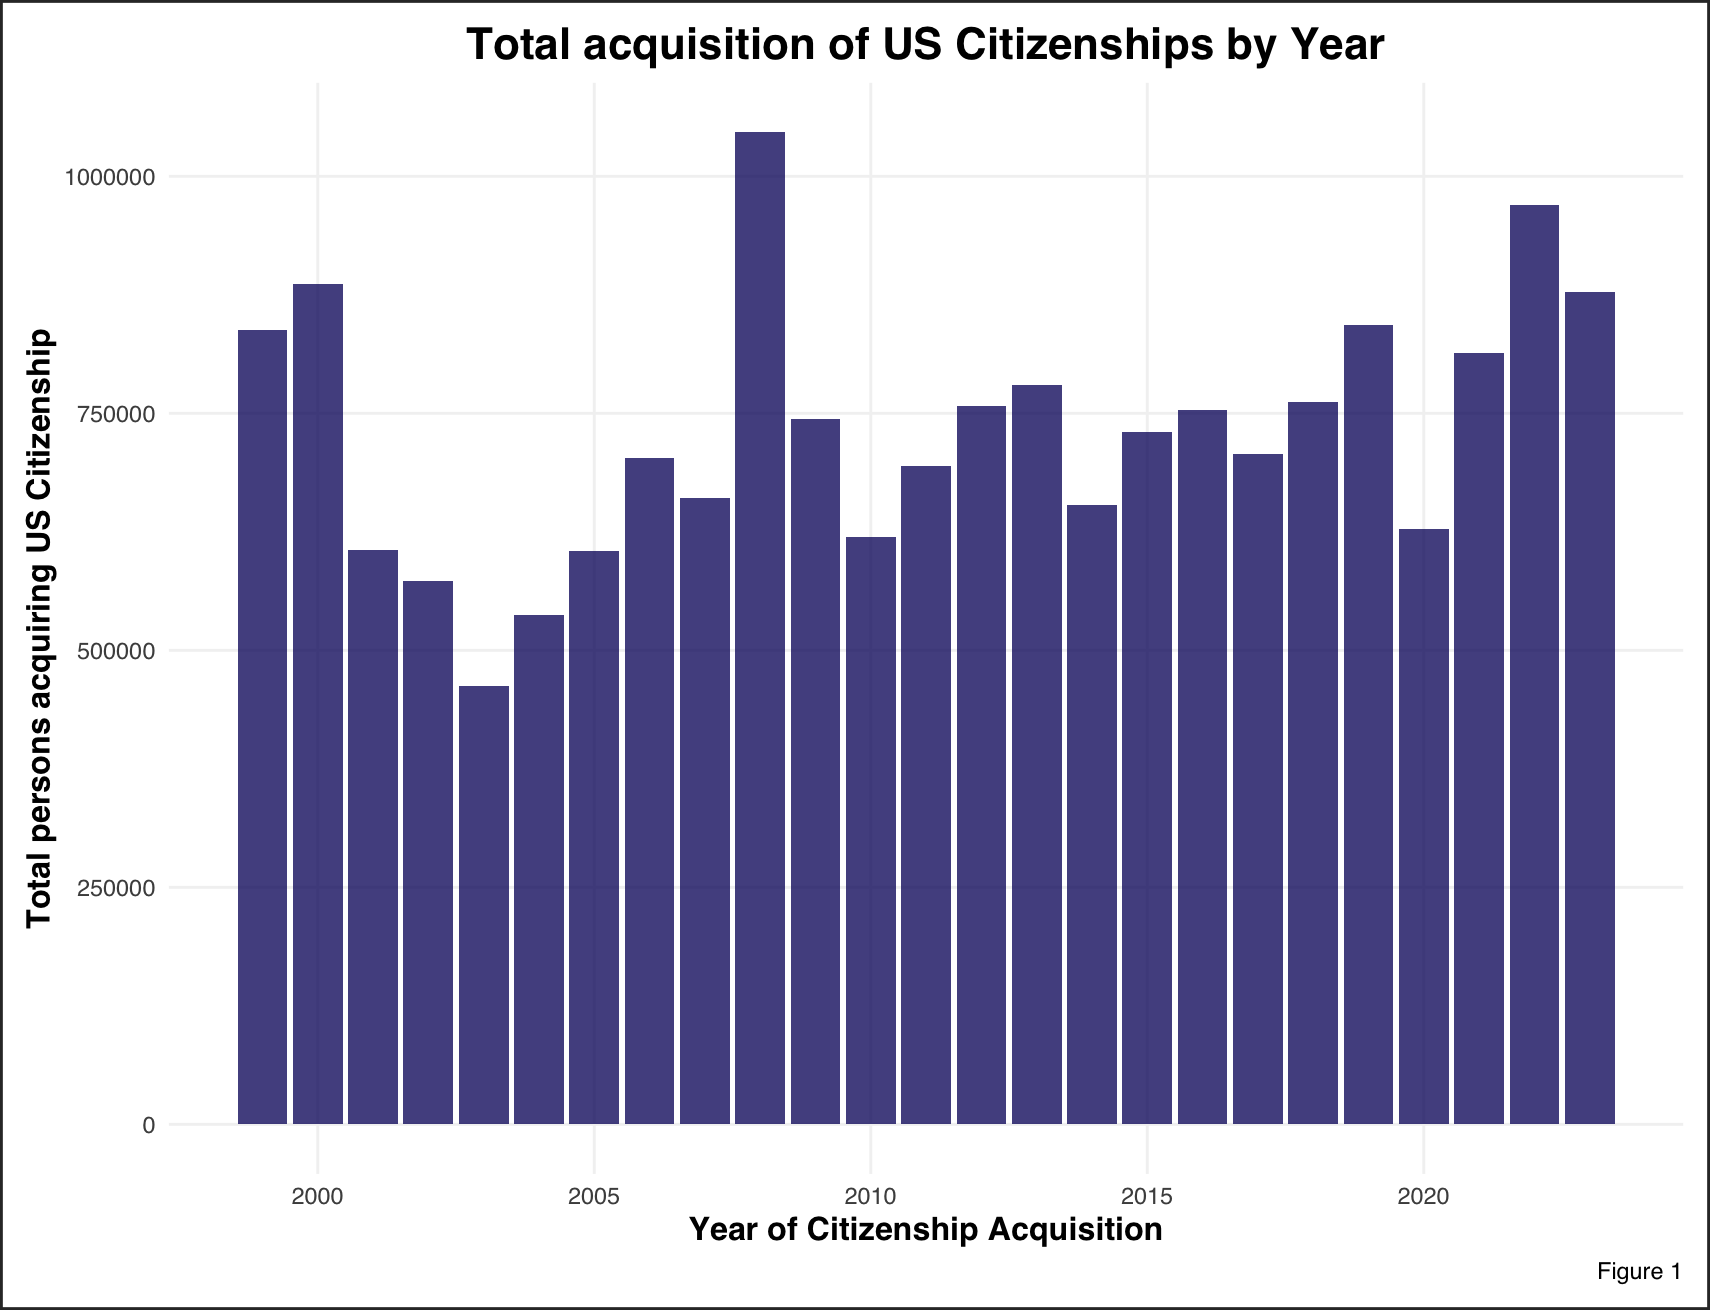
\includegraphics[width=0.8\textwidth]{figure_1.png}
\end{center}
The bar plot provides a high-level overview of US citizenship acquisitions, immediately revealing a massive, singular spike in 2008. While most years show a steady fluctuation between 500,000 and 800,000 acquisitions, the 2008 data point spikes over the rest, exceeding 1,000,000 persons. This outlier required a deeper investigation into which specific regions drove such a significant surge. This is what made me investigate and visualize figure 2, so I can understand which region has the major weight for this spike.
\VerbatimInput[firstline = 34, lastline = 51]{final_assignment_nk.R}

\subsection{Figure 2}
Here, I filtered the rows to get regions specified and the total number of persons. After the filter, the dataset included only the six primary geographic regions: Africa, Asia, Europe, the Americas, Oceania, and All other countries. I also did the same in pivoting the data to make it vertical instead of horizontal which helps in plotting it to understand the naturalization trends by region. 
\begin{center}
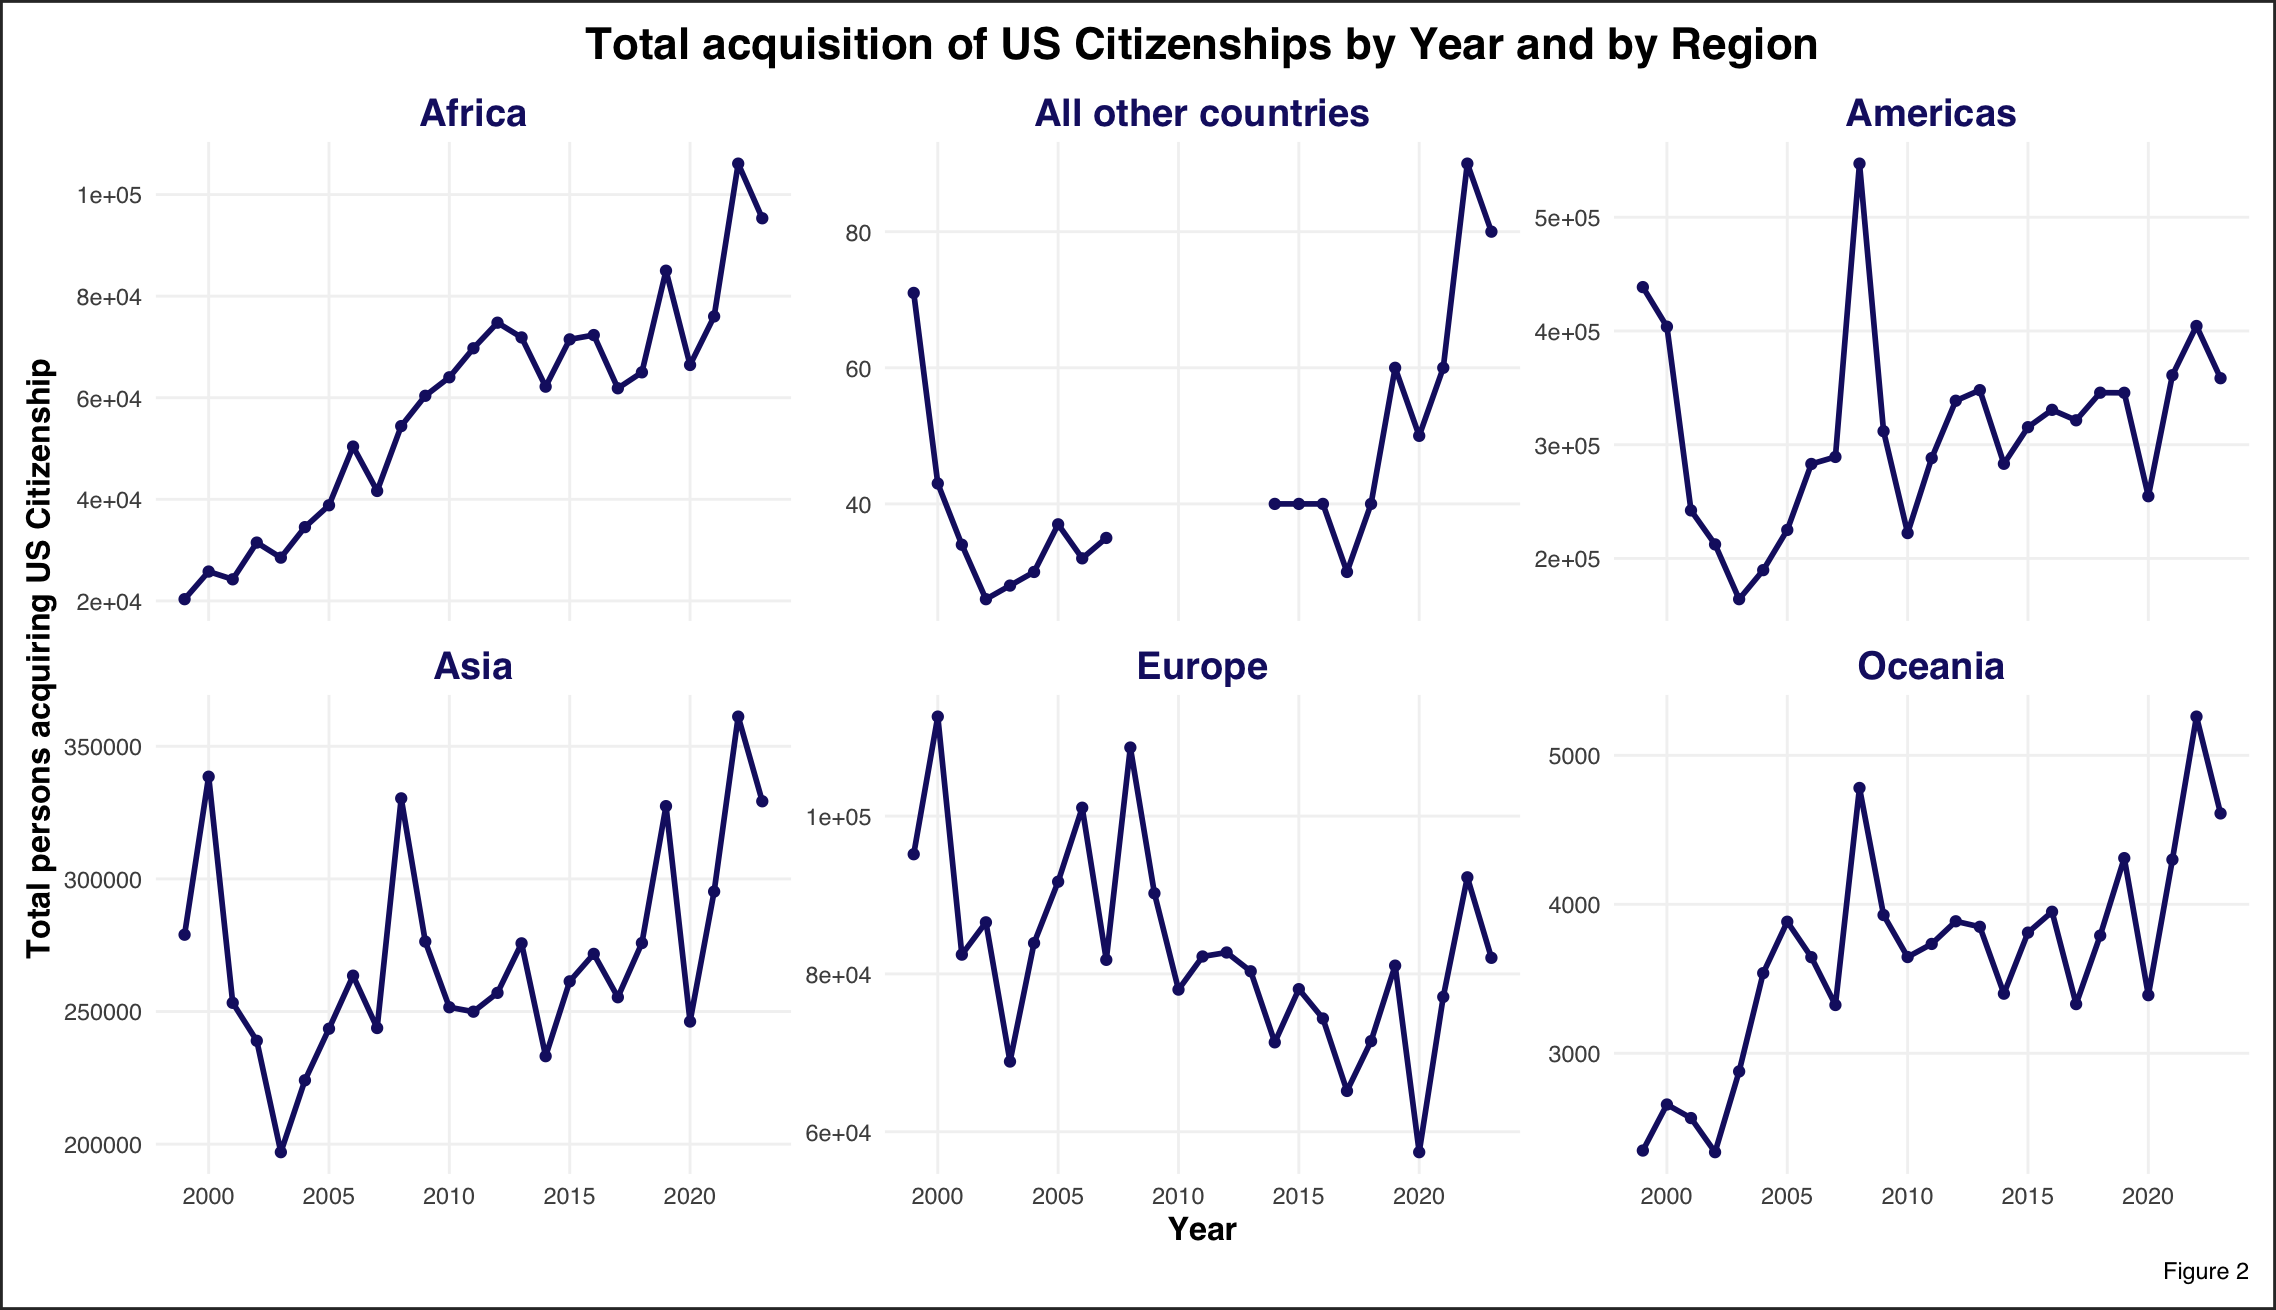
\includegraphics[width=0.8\textwidth]{figure_2.png}
\end{center}
While most regions experienced only slight fluctuations around 2008, the Americas plot displays a dramatic, sharp peak that mirrors the global spike. Acquisitions from the Americas nearly doubled during this window, jumping from approximately 300,000 to over 500,000. All regions show a peak or increases in trends per years and we can also see that each region has a range on the y-axis of persons acquiring the citizenship. My focus was to look at the trend in 2008 since this was the peak we saw in the first graph. We see that the peaks in 2008 are in Asia, Europe and Americas. But at the end, this regional analysis successfully narrows the search, confirming that the Americans was the primary driver of the global 2008 peak.
\VerbatimInput[firstline = 54, lastline = 77]{final_assignment_nk.R}

\subsection{Figure 3}
To find the reason behind the spike in Americas, I isolated the 2008 data for all countries within the Americas and joined it with global geographic coordinates. The resulting heat map uses color intensity to represent the volume of new citizens. I did the join by country in the USA, and set the location on the map using the longitude and the latitude. Then I plotted a heat map showing the naturalization trend or values in the USA countries.
\begin{center}
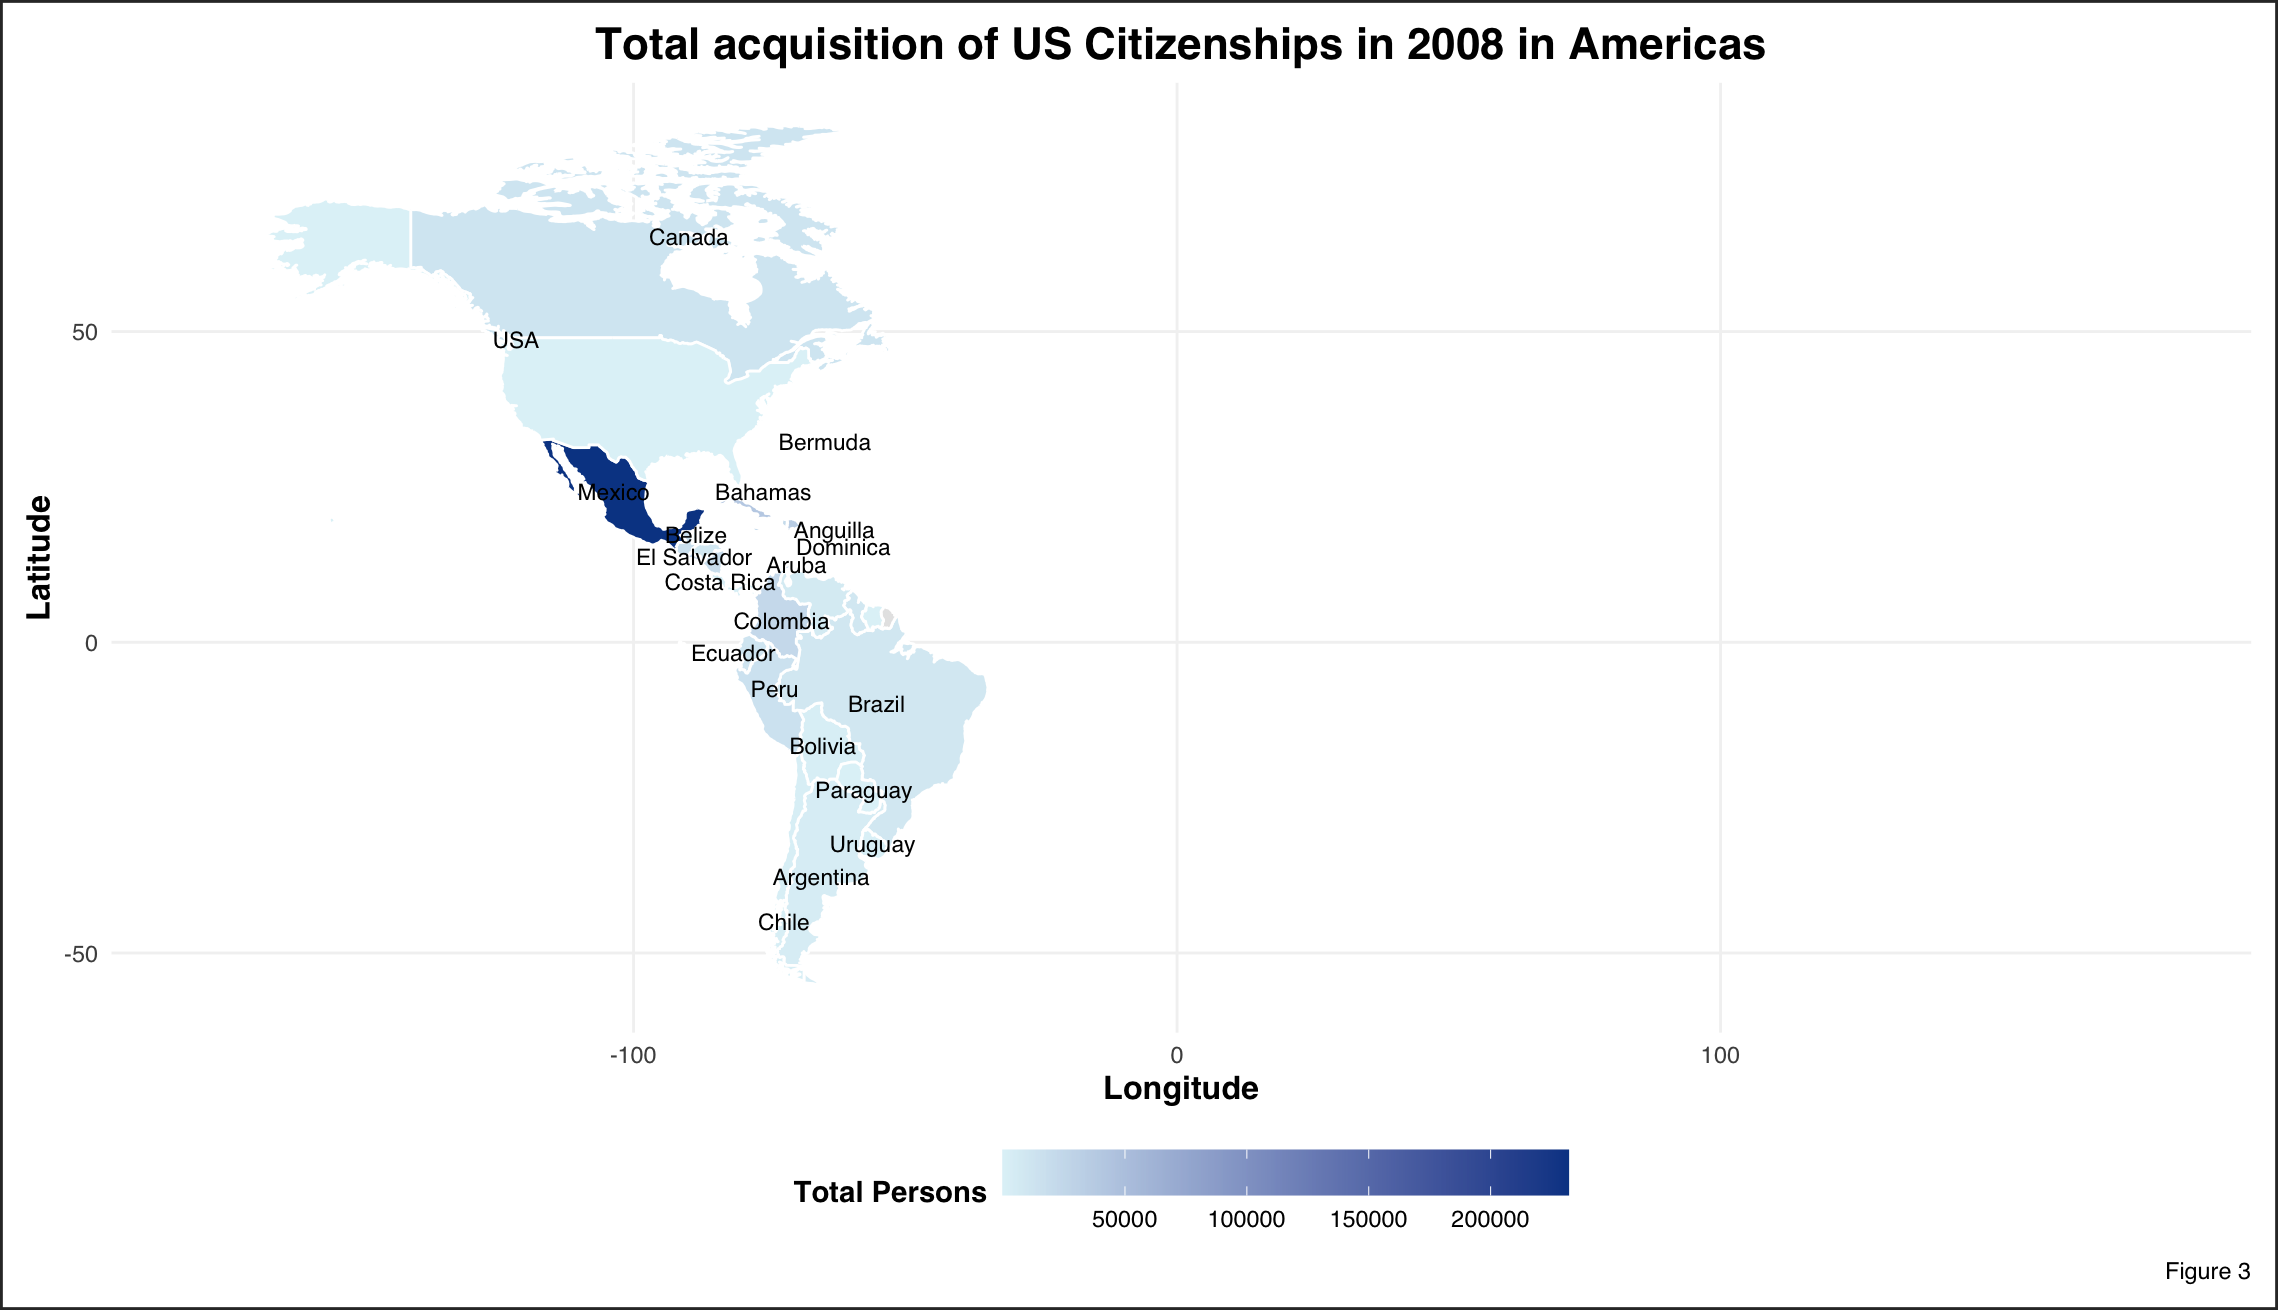
\includegraphics[width=0.8\textwidth]{figure_3.png}
\end{center}
While the United States and Canada appear in light blue (indicating moderate naturalization numbers), Mexico stands out in a deep midnight blue. This dark color immediately signals a massive statistical difference. The data confirms that Mexico’s naturalization count for 2008 exceeded 200,000 people, a figure that is significantly higher than any other neighboring nation in the Americas. By isolating this specific geographic data point, the heat map clearly identifies Mexico as the primary reason for the global spike seen in 2008. This increase was so large that it single-handedly changed the trend for the entire year, turning a period of steady growth into a historic anomaly.
\VerbatimInput[firstline = 81, lastline = 107]{final_assignment_nk.R}

\section{Conclusion}
As a conclusion, the data analysis journey reveals that the massive global spike in 2008 was not a uniform increase across all nations, but rather a concentrated surge originating within the Americas. By isolating this regional trend, the analysis identifies Mexico as the primary driver, with its record-breaking citizenship acquisitions single-handedly shifting the trajectory of the entire year's migration profile.

\end{document}